% Chapter 4

\chapter{Internship Subject} % Main chapter title

\label{Chapter3} % For referencing the chapter elsewhere, use \ref{Chapter3}

%----------------------------------------------------------------------------------------

% Define some commands to keep the formatting separated from the content
%\newcommand{\keyword}[1]{\textbf{#1}}
%\newcommand{\tabhead}[1]{\textbf{#1}}
%\newcommand{\code}[1]{\texttt{#1}}
%\newcommand{\file}[1]{\texttt{\bfseries#1}}
%\newcommand{\option}[1]{\texttt{\itshape#1}}

%----------------------------------------------------------------------------------------

\section{Problematics}

As I said in the previous parts, \iBubble{} includes a visual tracking system, \keyword{CMT}, to \emph{autonomously} follow divers underwater. This system currently uses \emph{openCV} libraries at a rate of \textbf{30 fps}. This speed can be improved using \emph{CUDA} technology. These features are only available on \keyword{BtB} versions of \iBubble{} fitted with \emph{Nvidia's Jetson embedded board}.

\keyword{BtC} versions of the drone uses \rasp{} in spite of the current \emph{Nvidia Graphics Card} wich means that \emph{CUDA} is no longer available because \vc{} is not designed with this technology.

As a consequence, \vc{} is not used so the whole tracking system is running only on the \cpu{} and the system rate drops to \textbf{7 fps}.

The more time-consuming part of the \keyword{CMT} is the \keyword{optical flow} computation. This is a fundamental tracking algorithm in Computer Vision. It uses \keyword{Gradient Descent} and \keyword{Pyramid} algorithms to get the displacement of the points of interest between two frames.

Therefore if we want to use the computing power of the \vc{}, it is compulsory to make our own implementation of the \keyword{optical flow} on \rasp, that was my internship subject.

The main difficulty is that there is no official \keyword{API} released by \textsc{Broadcom}. To compute the \keyword{optical flow} on \rasp, it was to necessary to follow the same steps as in Chapter~\ref{Chapter2}, namely:
\begin{itemize}
	\item write \code{code-to-execute} on \keyword{GPU} -- in \option{assembly language}
	\item parse this \code{code-to-execute} with \keyword{assembly parser} -- \file{qpu-asm.cpp}
	\item write a \code{driver program} for the \keyword{CPU} -- in \option{c-language}
	\item include this \keyword{API} in a \option{C++} project -- \keyword{CMT} is written in \option{C++}
\end{itemize}

%----------------------------------------------------------------------------------------

\section{Optical Flow}

Within \iBubble{} visual tracking system - \keyword{CMT} - \keyword{optical flow} is the displacement of points of interest - called \keyword{features} - between two consecutive frames from a video.

Computing \emph{optical flow} between two consecutive frames involves the following steps:
\begin{itemize}
	\item detect \keyword{features} on first image -- Figure~\ref{initFeaturesFig}
	\item find the next \keyword{features} positions on the second image -- Figure~\ref{secondFeaturesFig}
	\item compute \emph{displacemnt} for each \keyword{features} -- Figure~\ref{opticalFlowFig}
\end{itemize}


\begin{figure}[!htbp]
	\centering
	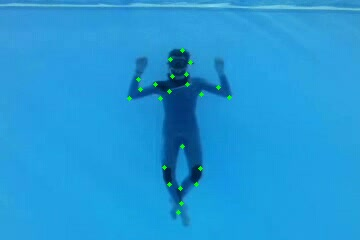
\includegraphics[width=0.5\textwidth]{plongeurInitFeatures}
	\caption{First frame of a diving video with the initial set of features}
	\label{initFeaturesFig}
\end{figure}
\FloatBarrier



\begin{figure}[!htbp]
	\centering
	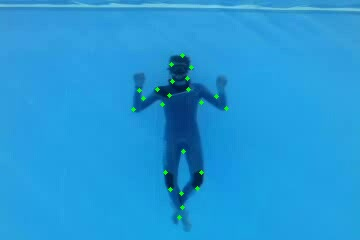
\includegraphics[width=0.5\textwidth]{plongeurNextFeatures}
	\caption{Second frame of a diving video with new features positions}
	\label{secondFeaturesFig}
\end{figure}
\FloatBarrier



\begin{figure}[!htbp]
	\centering
	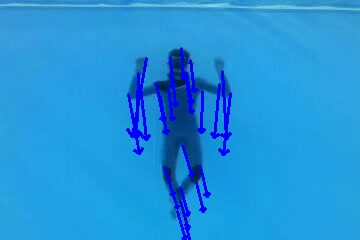
\includegraphics[width=0.5\textwidth]{plongeurOpticalFlow}
	\caption{Optical flow for the initial set of features -- \small{norm of the \textcolor{blue}{blue} vectors is overstated for better visualization}}
	\label{opticalFlowFig}
\end{figure}
\FloatBarrier

\emph{Optical flow} can be represented as a \emph{vector field}, representing \keyword{features} displacement between two consecutive frames. It is used to do object recognition, tracking or movement detection. In \iBubble, \emph{optical flow} is compute within \keyword{CMT} to achieve diver \emph{autonomous tracking and following}.\par

%----------------------------------------------------------------------------------------

\section{Lucas-Kanade method}

There are several ways to compute \keyword{optical flow}. Camille selected \keyword{Lucas-Kanade} method to be implemented on \vc.

\subsection{Images encodind}

As I mentioned in~\ref{Matrices}, frames from the \rasp{} camera are stored as \option{float-matrices} inside the shared RAM memory. Each \option{float value} is a 32-bit word All the algorithms described below are using grayscale images. That means that all
images contain pixels that have a single intensity channel (generally encoded as float 32 bits).

Frames dimensions are 240X360. It is row major.

\[
\begin{bmatrix}
pixel_{0,0} & pixel_{0,1} & \ldots & pixel_{0,359}\\
pixel_{1,0} & \ddots & \ldots & pixel_{1,359}\\
\vdots & \vdots & \ddots & \vdots\\
pixel_{239,0} & \ldots & \ldots & pixel_{239,359}
\end{bmatrix}_{240\times 360}
\]

%----------------------------------------------------------------------------------------

\section{Implementation on \vc}

%----------------------------------------------------------------------------------------
